% HEADER
\documentclass[class=article, crop=false]{standalone}
\usepackage{00_Preamble/frr_preamble}

% Packages
\usepackage{titlesec}	
\usepackage{hyperref}
\usepackage{float}
\usepackage{graphics}
\usepackage{placeins}
\usepackage{adjustbox}
% END HEADER

\begin{document}
	\section{Payload Criteria}
%	Payload Design
%	Describe any changes in the payload design form CDR, and why those changes are necessary
%	Describe unique features of the payload
%	Structural elements
%	Electrical elements
%	Drawings and schematics of the as built payload
%	Discuss flight reliability confidence. Demonstrate that the design can meet mission success criteria
%	Prove that the payload is fully constructed, and fully document the construction process
%	Include schematics of the AS BUILT payload. There is a good chance dimensions will change slightly due to construction.
%	Discuss how and why the constructed payload differs from earlier models.
	
		% HEADER
\documentclass[class=article, crop=false]{standalone}
\usepackage{00_Preamble/frr_preamble}

% Packages
\usepackage{titlesec}
\usepackage{hyperref}
\usepackage{float}
\usepackage{graphics}
\usepackage{placeins}
\usepackage{adjustbox}
% END HEADER

\begin{document}
	\subsection{Payload Summary}
	\label{subsec:payload_summary}
	\subsubsection{Mission Statement and Success Criteria}
	\paragraph{Mission Statement}
	The mission of the VADL 2017-2018 payload is to perform target detection through real-time image capturing and processing. Sectional roll control facilitates the imaging system by compensating for natural roll. This allows the payload to reorient itself to take pictures of targets as the rocket is in ascent, rather than simply having the targets move in and out of the image frame.
	
	\paragraph{Mission Success Criteria}
	For the mission to be a success, it must be conducted in accordance with all NASA and range imposed requirements and regulations, particularly with respect to safety. The following mission success criteria are not exhaustive in nature and only apply to the payload system. Vehicle and recovery success criteria are found in Section \ref{subsubsec:vehicle_mission_success_criteria}. A more exhaustive list of mission success criteria is found in Section \ref{subsec:requirements_compliance}. Sections concerning the payload's physical layout (Section \ref{subsec:payload_layout}), hardware (Section \ref{subsec:payload_hardware}), and software (Section \ref{subsec:payload_software}) demonstrate the fulfillment of payload mission success criteria.
	
	\paragraph{SL Payload Mission Success Criteria} 
	\begin{itemize}
		\item Teams will design an on-board camera system capable of identifying and differentiating between 3 randomly placed targets.
		\item Data from the camera system will be analyzed in real time by a custom designed on-board software package that shall identify and differentiate between the three targets.
		
	\end{itemize}
	
	\paragraph{Team Derived Payload Mission Success Criteria} 
	\begin{itemize}
		\item Distance and location of the target in the image shall be obtained via edge detection and color matching.
		\item Imaging and target detection shall still be completed upon loss of motor control.
		\item The SRC motor shall use imaging data as a reference input to control the induced roll of the fore-section.
		\item Angular position of the forward section of the rocket shall be controlled by a motor to within 3 degrees.						
	\end{itemize}

	\pagebreak
	
	\subsubsection{Payload Overview}
	The payload will be comprised of two interconnected subsystems: an imaging system and a Brushless DC (BLDC) motor control system. Target detection will be performed by the imaging system, and the output of that system's analysis will inform the setpoint of the BLDC motor control system. The key innovation of this vehicle and payload is Sectional Roll Control (SRC) - a mechanism that allows decoupling of the aft and fore sections of the rocket, with angular position control of the fore section. SRC enables the real-time imaging data not only to be recorded, but also to influence the vehicle's positioning in order to improve imaging of targets. This innovation closes the loop and justifies real-time image processing.
	
	\bigbreak
	
	%reference block diagram figure
	\FloatBarrier
	\begin{figure}[!h]
		\centering
		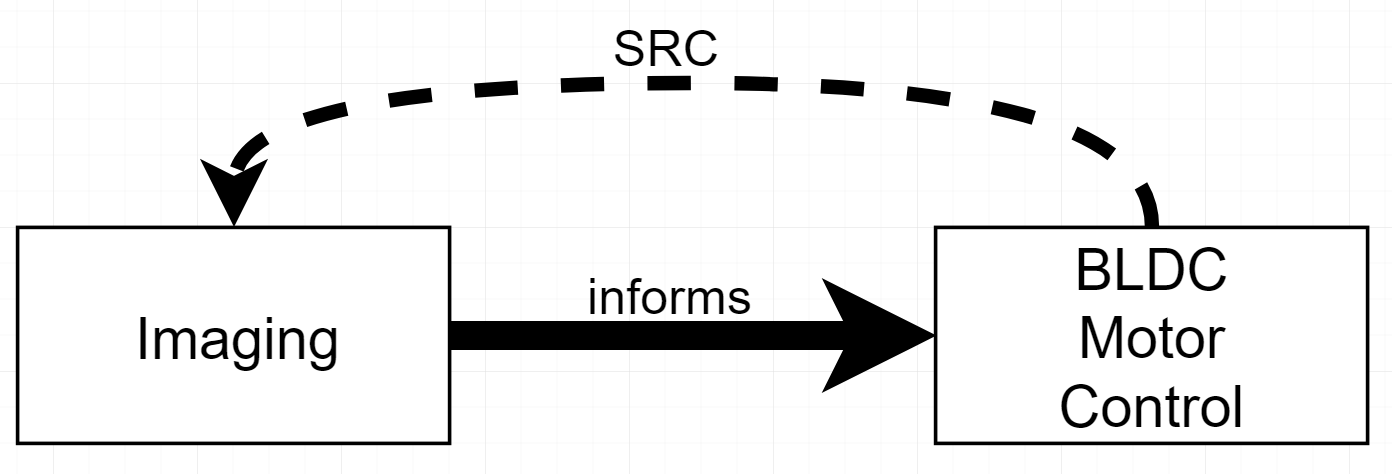
\includegraphics[width=.7\linewidth]{09_Figures/Payload-Summary-Block-Diagram.png}
		\caption{Payload Flow of Influence}
		\label{fig:Payload-Summary-Block-Diagram}
	\end{figure}
	\FloatBarrier
	
	The imaging system will have two cameras to increase field of view and improve reliability. Each camera will have a dedicated Image Processing Unit (IPU). For each image taken, the IPUs will determine if the target is in the frame of the image. If the target is found by one of the cameras, the location of the target in the frame and the pixel size of the target will be processed in order to determine the desired change in the angular position of the fore section. The motor control system then attempts to reach that setpoint. This system control flow from sensors to actuator is shown in Figure \ref{fig:payloadWOO}.
	
	\bigbreak
	
	The multiple processing systems on board will allow for concurrency in computation and real-time target tracking and mechanical response. ``Real-time" computing systems guarantee a correct system response within a specified time constraint. For this application, a ``real-time" response is defined by the window of the flight experiment. This payload's image processing system has hard real-time requirements because of the short experimental window in which SRC actuation must center targets in the field of view of one of its cameras.
	
	\bigbreak
	
	The entire payload will operate in a continuous loop for the duration of the experimental window.
	
	\bigbreak
	
	%payloadWOO figure blows their minds! Oh God! Its so bloody!
	\FloatBarrier
	\begin{figure}[!h]
		\centering
		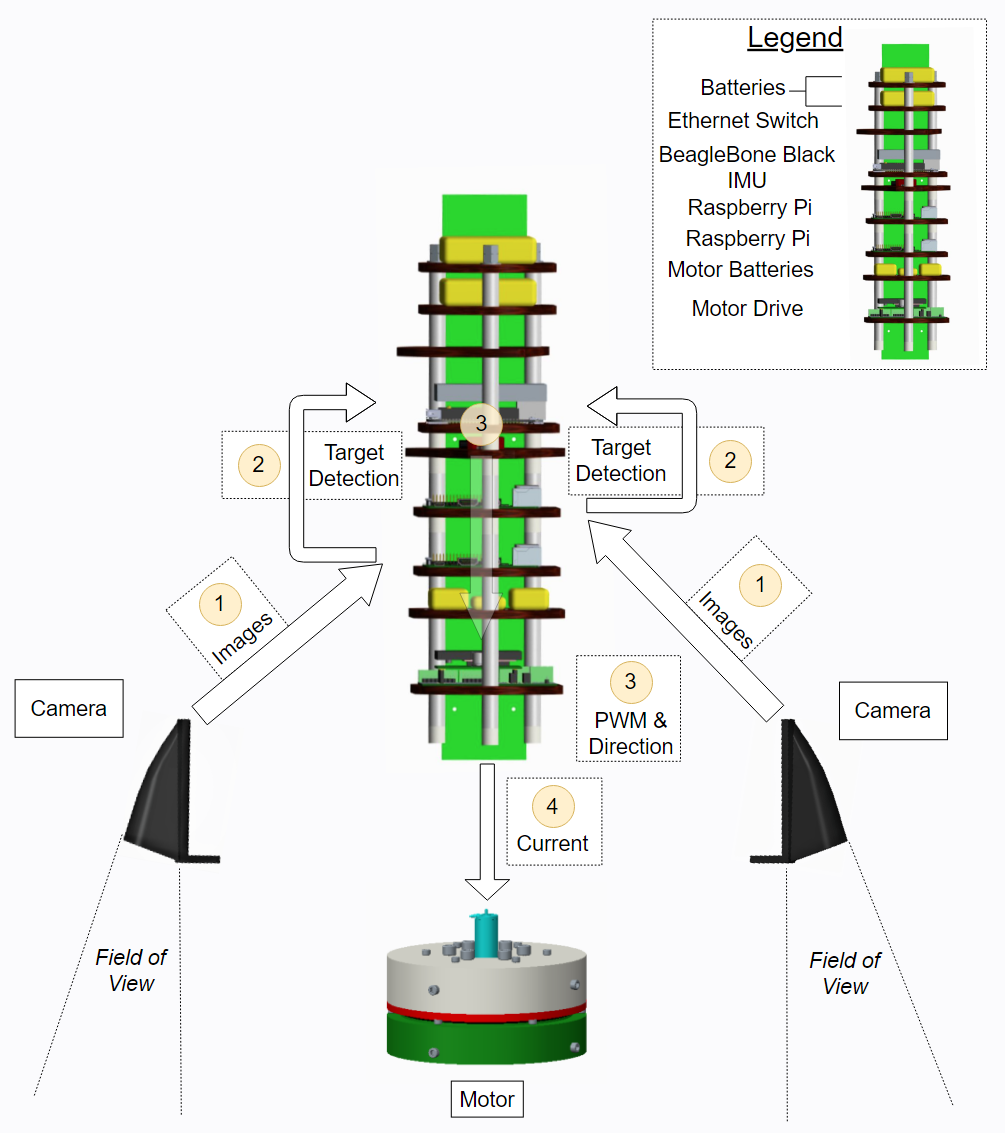
\includegraphics[width=0.85\linewidth]{09_Figures/Payload/payloadWOO.png}
		\caption{Exploded View of Payload with Dataflow Overlay}
		\label{fig:payloadWOO}
	\end{figure}
	\FloatBarrier
	
\end{document}

		\pagebreak
		
		% HEADER
\documentclass[class=article, crop=false]{standalone}
\usepackage{00_Preamble/frr_preamble}

% Packages
\usepackage{titlesec}	
\usepackage{hyperref}
\usepackage{float}
\usepackage{graphics}
\usepackage{placeins}
\usepackage{adjustbox}
% END HEADER

\begin{document}
	\subsection{Layout}
	\label{subsec:payload_layout}
	\subsubsection{Full Assembly}
	The payload assembly is located in the fore section of the vehicle. As shown in Figure \ref{fig:360access}, the payload components are mounted along three threaded rods. These rods anchor into the SRC mechanism, connecting the payload to the vehicle. Payload components are attached to laser cut, 0.25" Baltic birch plywood shelves. Each shelf is customized in shape to meet the needs of its components, while maintaining at least three points of contact to the carbon fiber body tube. This allows every shelf to act as a centering bulkhead to prevent lateral movement of the payload.
	
	\bigbreak
	
	% \FloatBarrier
	% \begin{figure}[!h]
	% \captionsetup[subfigure]{justification=centering}
	% \centering
	% \begin{subfigure}{.45\textwidth}
	% \centering
	% \includegraphics[width=0.4\linewidth]{09_Figures/Payload/FullAssembly1.jpg}
	% \caption{CAD of full Payload Assembly}
	% \label{fig:payloadFullCAD}
	% \end{subfigure}
	% \begin{subfigure}{.45\textwidth}
	% \centering
	% \includegraphics[width=0.4\linewidth]{09_Figures/Payload/payloadOnSRC.png}
	% \caption{Payload with SRC and Camera Shrouds}
	% \label{fig:payloadOnSRC}
	% \end{subfigure}
	% \caption{CAD and Picture of Payload Assembly with SRC Mechanism and Camera Shrouds}
	% \label{fig:fullPayloadYeah}
	% \end{figure}
	% \FloatBarrier
	
	\FloatBarrier{}
	\begin{figure}[!h]
		\centering
		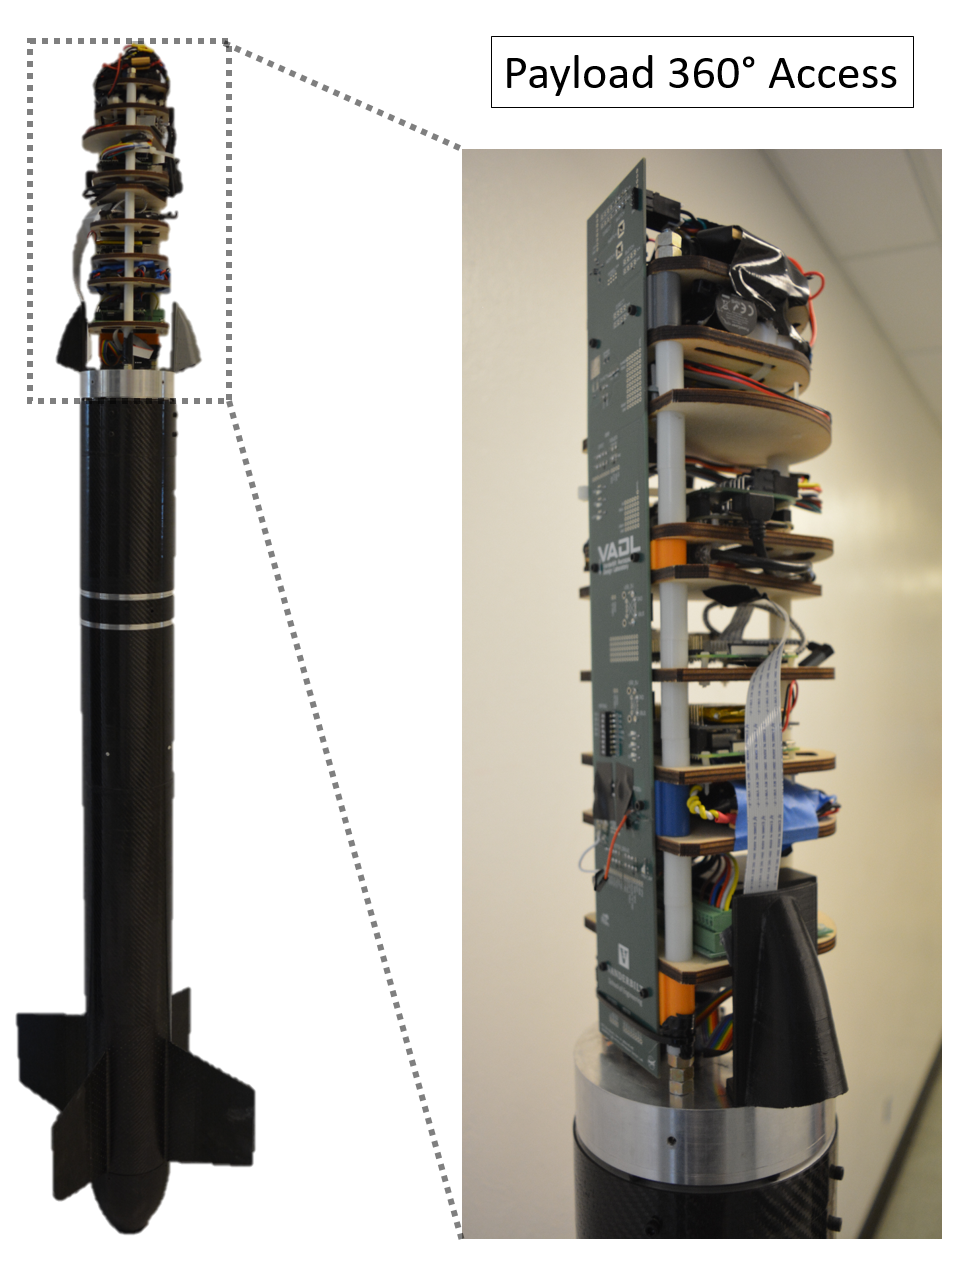
\includegraphics[width=0.7\linewidth]{09_Figures/Payload/360access.png}
		\caption{Flight-Ready Payload on Vehicle}
		\label{fig:360access}
	\end{figure}
	\FloatBarrier{}
	
	This physical layout offers a distinct advantage over the previous design in that it provides full access to all payload components and connections throughout assembly. As Figure \ref{fig:360access} illustrates, the launch vehicle with payload can reach the stage of full assembly before the nosecone and fore section carbon fiber tube are attached. This creates the opportunity to visually verify that all electrical and mechanical connections are satisfactory on the launchpad. Additionally, arming of payload power switches, experiment deployment over ethernet, and confirmation of status LEDs can be performed without any accessibility cut-outs in the vehicle body.
	
	% \FloatBarrier{}
	% \begin{figure}[!h]
	% \centering
	% \captionsetup{justification=centering}
	% \includegraphics[width=0.7\linewidth]{09_Figures/Payload/payloadFullOnLaunchpad.png}
	% \caption{Vehicle and Payload Configuration on Launchpad. \\ Design provides complete access to payload. \\ REPLACE WITH ACTUAL PHOTO!!!!!!!!!!!}
	% \label{fig:payloadFullOnLaunchpad}
	% \end{figure}
	% \FloatBarrier{}
	
	% Replaced by above figure with callout
%	\FloatBarrier
%	\begin{figure}[!h]
%		\captionsetup[subfigure]{justification=centering}
%		\centering
%		\begin{subfigure}{.58\textwidth}
%			\centering
%			\includegraphics[width=0.58\linewidth]{09_Figures/Payload/fullOnPadCAD.jpg}
%			\caption{CAD Model}
%			\label{fig:fullOnPadCAD}
%		\end{subfigure}
%		\begin{subfigure}{0.37\textwidth}
%			\centering
%			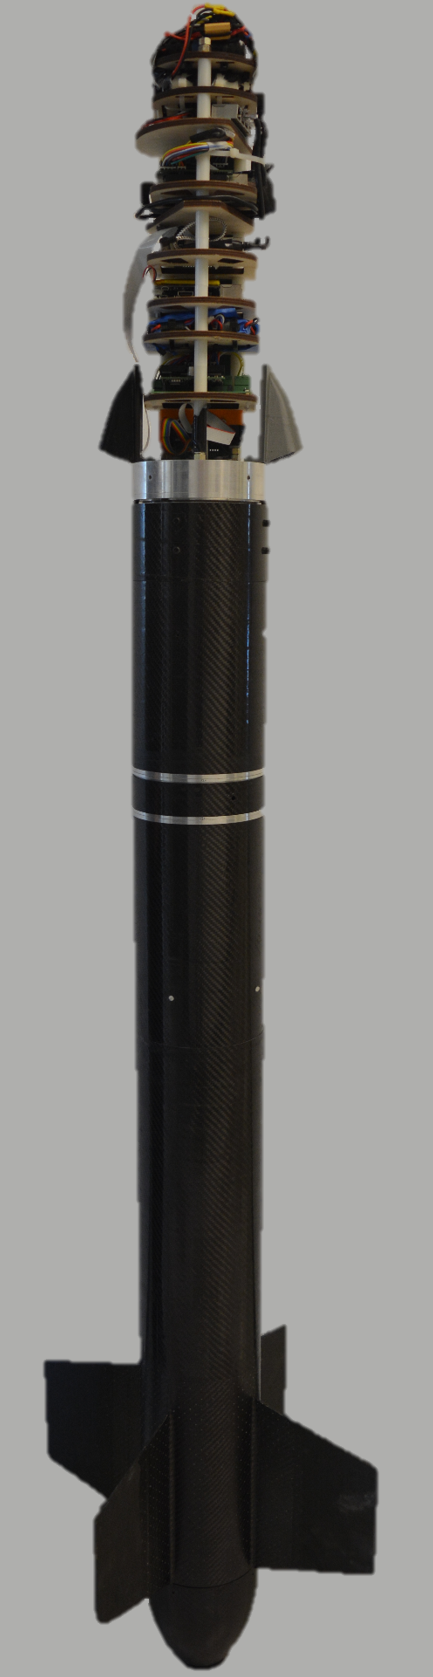
\includegraphics[width=0.37\linewidth]{09_Figures/Payload/360_final.png}
%			\caption{As Built}
%			\label{fig:360_final}
%		\end{subfigure}
%		\caption{Vehicle and Payload Launchpad Configuration}
%		\label{fig:fullVehicleAndPayloadPad}
%	\end{figure}
%	\FloatBarrier
	
	%%%%% MECHANICAL DRAWING OF SHELF STACKUP %%%%%%%%%%%%%%%%%
	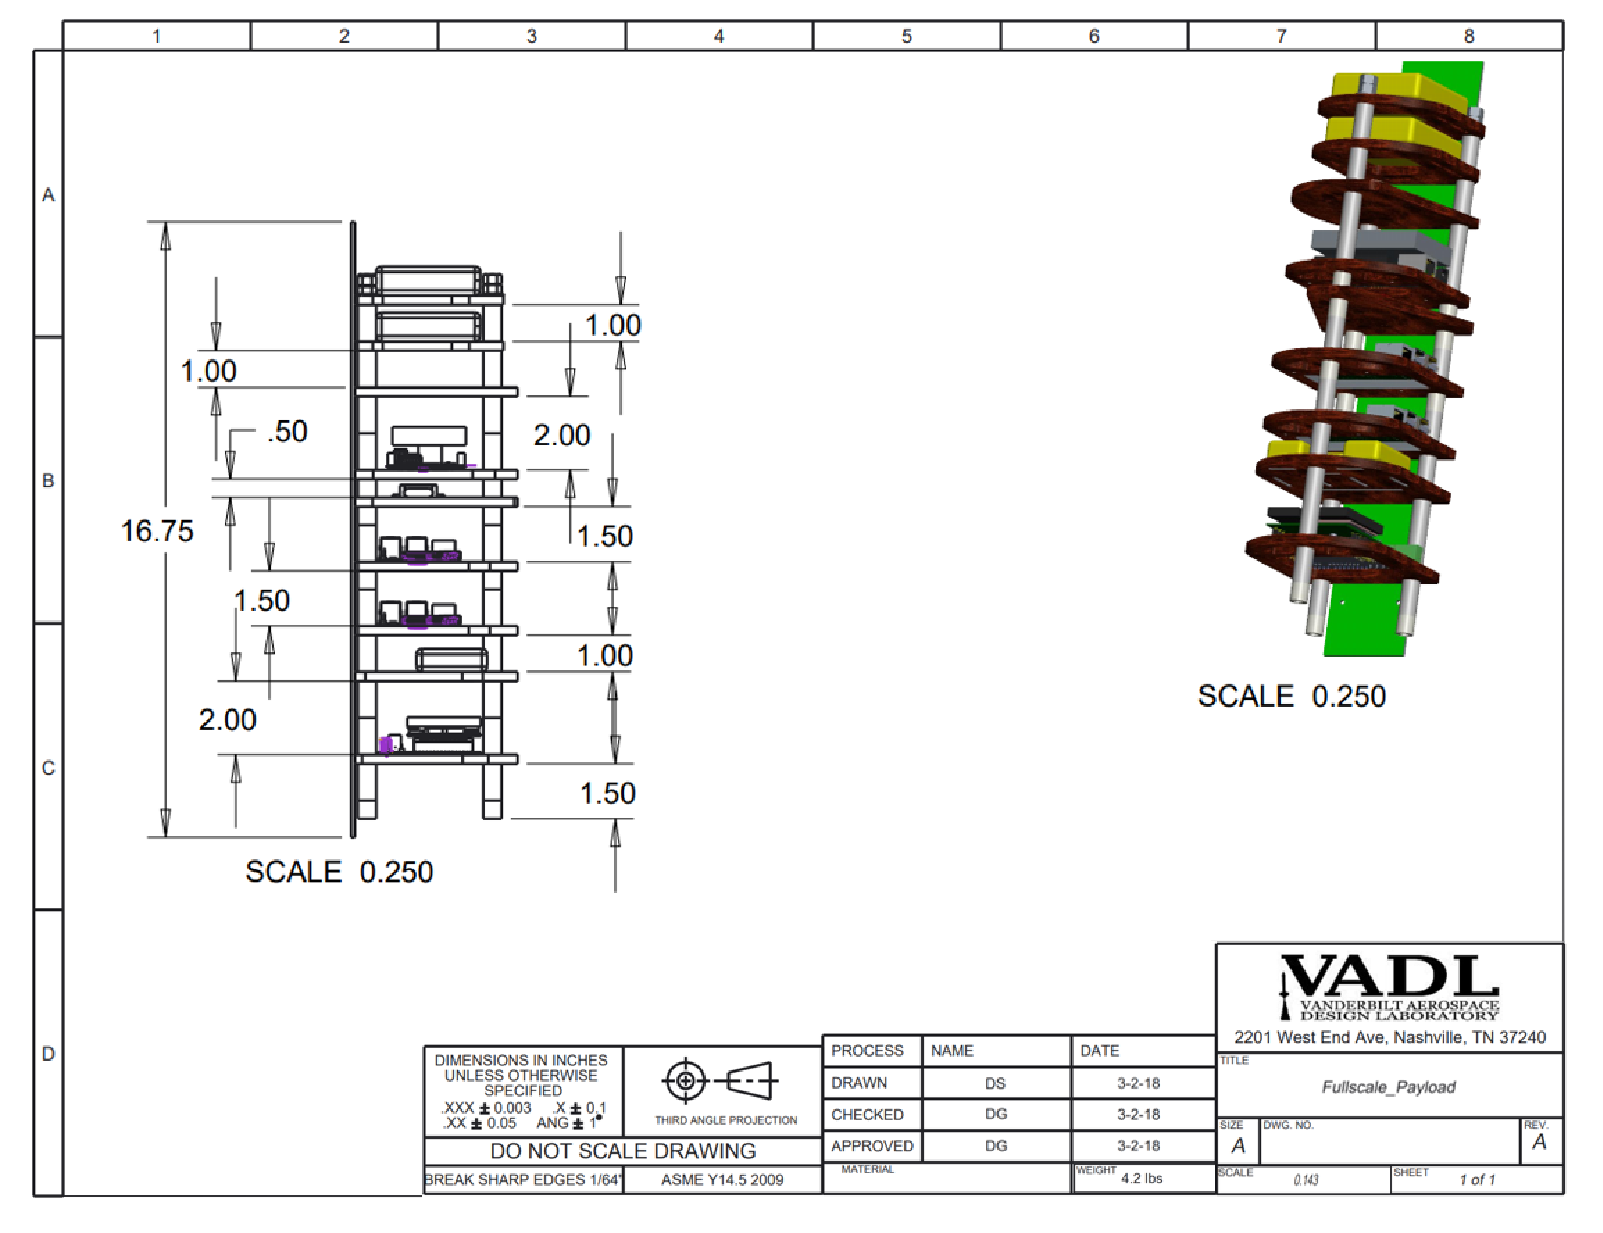
\includepdf[pages=-, pagecommand={}]{09_Figures/Payload/final_drawing1}
	
	\subsubsection{Vehicle Integration}
	
	\paragraph{Connection to SRC Mechanism}
	\label{paragraph:payload_to_src}
	The physical connection of the stepped payload to the surface of the SRC mechanism will occur using a simple threaded connection through the SRC surface with the payload's threaded rods. This surface will offer approximately 5 threads of engagement to the rods, which would most likely be more than sufficient. However, to help mitigate risk associated with vibration, jam nuts will be placed above and below that surface in order to further prevent motion along the rocket's axis. Should this prove insufficient, the threaded rods may be permanently installed using Loctite.
	
	\bigbreak
	
	\FloatBarrier{}
	\begin{figure}[!h]
		\centering
		\includegraphics[width=0.46\linewidth]{09_Figures/Payload/SRCwithShrouds.png}
		\caption{Threaded rods and camera shrouds mounted into SRC}
		\label{fig:payloadConnectSRC}
	\end{figure}
	\FloatBarrier{}
	
	% \FloatBarrier
	% \begin{figure}[!h]
	% \captionsetup[subfigure]{justification=centering}
	% \centering
	% \begin{subfigure}{.45\textwidth}
	% \centering
	% \includegraphics[width=0.4\linewidth]{09_Figures/Payload/NewSRC_w_Shrouds.jpg}
	% \caption{Threaded rods and camera shrouds mounted into SRC}
	% \label{fig:payloadConnectSRC}
	% \end{subfigure}
	% \begin{subfigure}{.45\textwidth}
	% \centering
	% \includegraphics[width=0.4\linewidth]{09_Figures/Payload/newSRCwithShrouds.png}
	% \caption{BLAH}
	% \label{fig:payloadConnectSRC_real}
	% \end{subfigure}
	% \caption{BLAH}
	% \label{fig:payloadConnect}
	% \end{figure}
	% \FloatBarrier
	
	\paragraph{Camera Shrouds}
	\label{paragraph:shroud_design}
	
	The payload requirements for this design dictate that two redundant cameras be mounted externally from the rocket, diametrically opposed. This requirement necessitates the design of aerodynamic shrouds, which simultaneously position the cameras with a maximum field of view for target detection, protect the cameras during flight, and minimally increase the drag coefficient of the rocket. Figure \ref{fig:shroudINTHEREAL} shows the shroud design.
	
	\bigbreak
	
	
	\FloatBarrier
	\begin{figure}[h]
		\centering
		\includegraphics[width=0.21\linewidth]{09_Figures/Payload/camShroud.png}
		\caption{3D-printed Camera Shroud}
		\label{fig:shroudINTHEREAL}
	\end{figure}
	\FloatBarrier
	
	The payload cameras are housed by aerodynamic shrouds mounted directly on the SRC mechanism. The shrouds are each affixed by two 6-32 screws, and designed to align on the outer edge of the SRC mechanism. The carbon fiber body will slide over the shrouds and be bolted to the SRC mechanism.
	
	
	\bigbreak
	The camera shrouds are designed to allow mounting of the cameras on an angled plane internal to the camera shroud. This angle is determined by the angle of the camera's vertical field of view, maximizing the field of view of the cameras. The cameras will be bolted to the plane using 4 threaded aluminum 2-56 bolts and nuts.
	
	\bigbreak
	
\end{document}

		\pagebreak
		
\end{document}
